\section{Curvature-defined EDT window in K$_3$C$_{60}$}

K$_3$C$_{60}$ is a useful materials test case for the present diagnostic because it combines narrow near-Fermi bands with strong electron--phonon coupling in a molecular solid, so finite non-adiabatic structure is expected without having to invoke a broad many-parameter model~\cite{Gunnarsson1997,Capone2009}. In the present manuscript, K$_3$C$_{60}$ is the main material example used to anchor EDT to a falsifiable microscopic quantity rather than to a qualitative narrative. The role of Fig.~\ref{fig:k3c60_edt_window} is therefore specific: it shows exactly which curvature pair is analyzed, how the local quadratic window is extracted, and how sensitive the extracted window is to analysis choices. The Supplement places this main example in a broader archived-controls context using representative comparison datasets from V, Na, LaH$_{10}$, and YBa$_2$Cu$_3$O$_7$.

The reproducible bundle for this case study contains two complementary data products. Panel (a) uses the archived near-Fermi band-structure figure \texttt{figures/supplementary/K3C60-bands.pdf} as band-context reference for the same calculation. Panels (b)--(e) are generated directly from the bundled curvature export \texttt{data/k3c60/tmp.agr} by running \texttt{python scripts/make\_fig2\_k3c60\_edt.py}. The metadata embedded in the AGR file identify the observable as a mode-resolved curvature trace, $\partial^2 E_n(k)/\partial q^2$, evaluated along the $\Gamma$--X--L--W--$\Gamma$ path. The archived companion figure and caption identify the representative normal mode as \texttt{m120} at $1090.35~\mathrm{cm}^{-1}$.

Curvature is extracted from displaced electronic-structure calculations as the second derivative of the band energy with respect to phonon normal-mode coordinate, as defined in the preceding curvature-diagnostic section; the bundled archive provides the resulting mode-resolved curvature traces rather than the full family of displaced calculations. Within that exported dataset, we analyze Bands 208 and 209 in the archived numbering because they form the clearest opposite-sign branch pair in the selected momentum interval. Operationally, the pair is identified by locating a local minimum in one branch and a local maximum in the other at the same momentum point inside the analysis window. For the nominal window used in Fig.~\ref{fig:k3c60_edt_window}, both extrema occur near $k \approx 0.818$, and the corresponding local quadratic fits give a shared center $k_0 = 0.823$.

The finite EDT window is then defined from the paired-branch residual diagnostic. Using the analysis slice indexed by 150--281 in the archived trace, a nominal local fit half-window of 18 points, and a residual threshold $R_{\rm th}=0.08$, we obtain a finite window extending from $k_{\rm left}=0.742$ to $k_{\rm right}=0.896$, corresponding to $\Delta k_{\rm EDT}=0.154$. Panel (d) makes this definition explicit by plotting the branch-resolved residuals and shading the interval over which the two branches remain simultaneously compatible with the local quadratic description. This is the quantity we use as the curvature-defined EDT window in the K$_3$C$_{60}$ analysis.

The main robustness checks are summarized in panel (e) and in Supplementary Fig.~S5. Varying the residual threshold from 0.04 to 0.18 changes the extracted width only from 0.137 to 0.178, while varying the fit-window size from 10 to 28 points changes the width from 0.127 to 0.199. Subsampling the $k$ grid from 131 points down to 33 points gives widths between 0.144 and 0.164. A local-fit bootstrap around the selected pair gives a 95\% confidence interval of $[0.147,\,0.158]$ for the nominal width. We also compare neighboring band-pair choices, which shows that pair selection is a real analysis axis rather than a hidden fixed choice: the archived visible pair, Bands 208/209, gives the nominal window, while nearby pairs give different finite widths. The only robustness axis that cannot be reproduced from the bundled archive is a displacement-amplitude sweep, because the archived dataset contains one exported curvature product rather than a matched family of displaced calculations at multiple amplitudes. This is why the supplementary cross-material datasets are interpreted conservatively as diagnostic portability checks based on explicit representative candidate pairs, rather than as material-by-material reconstructions with identical evidentiary weight.

\begin{figure*}[t]
\centering
\begin{minipage}{0.48\linewidth}
\textbf{(a)}\\[-0.4em]
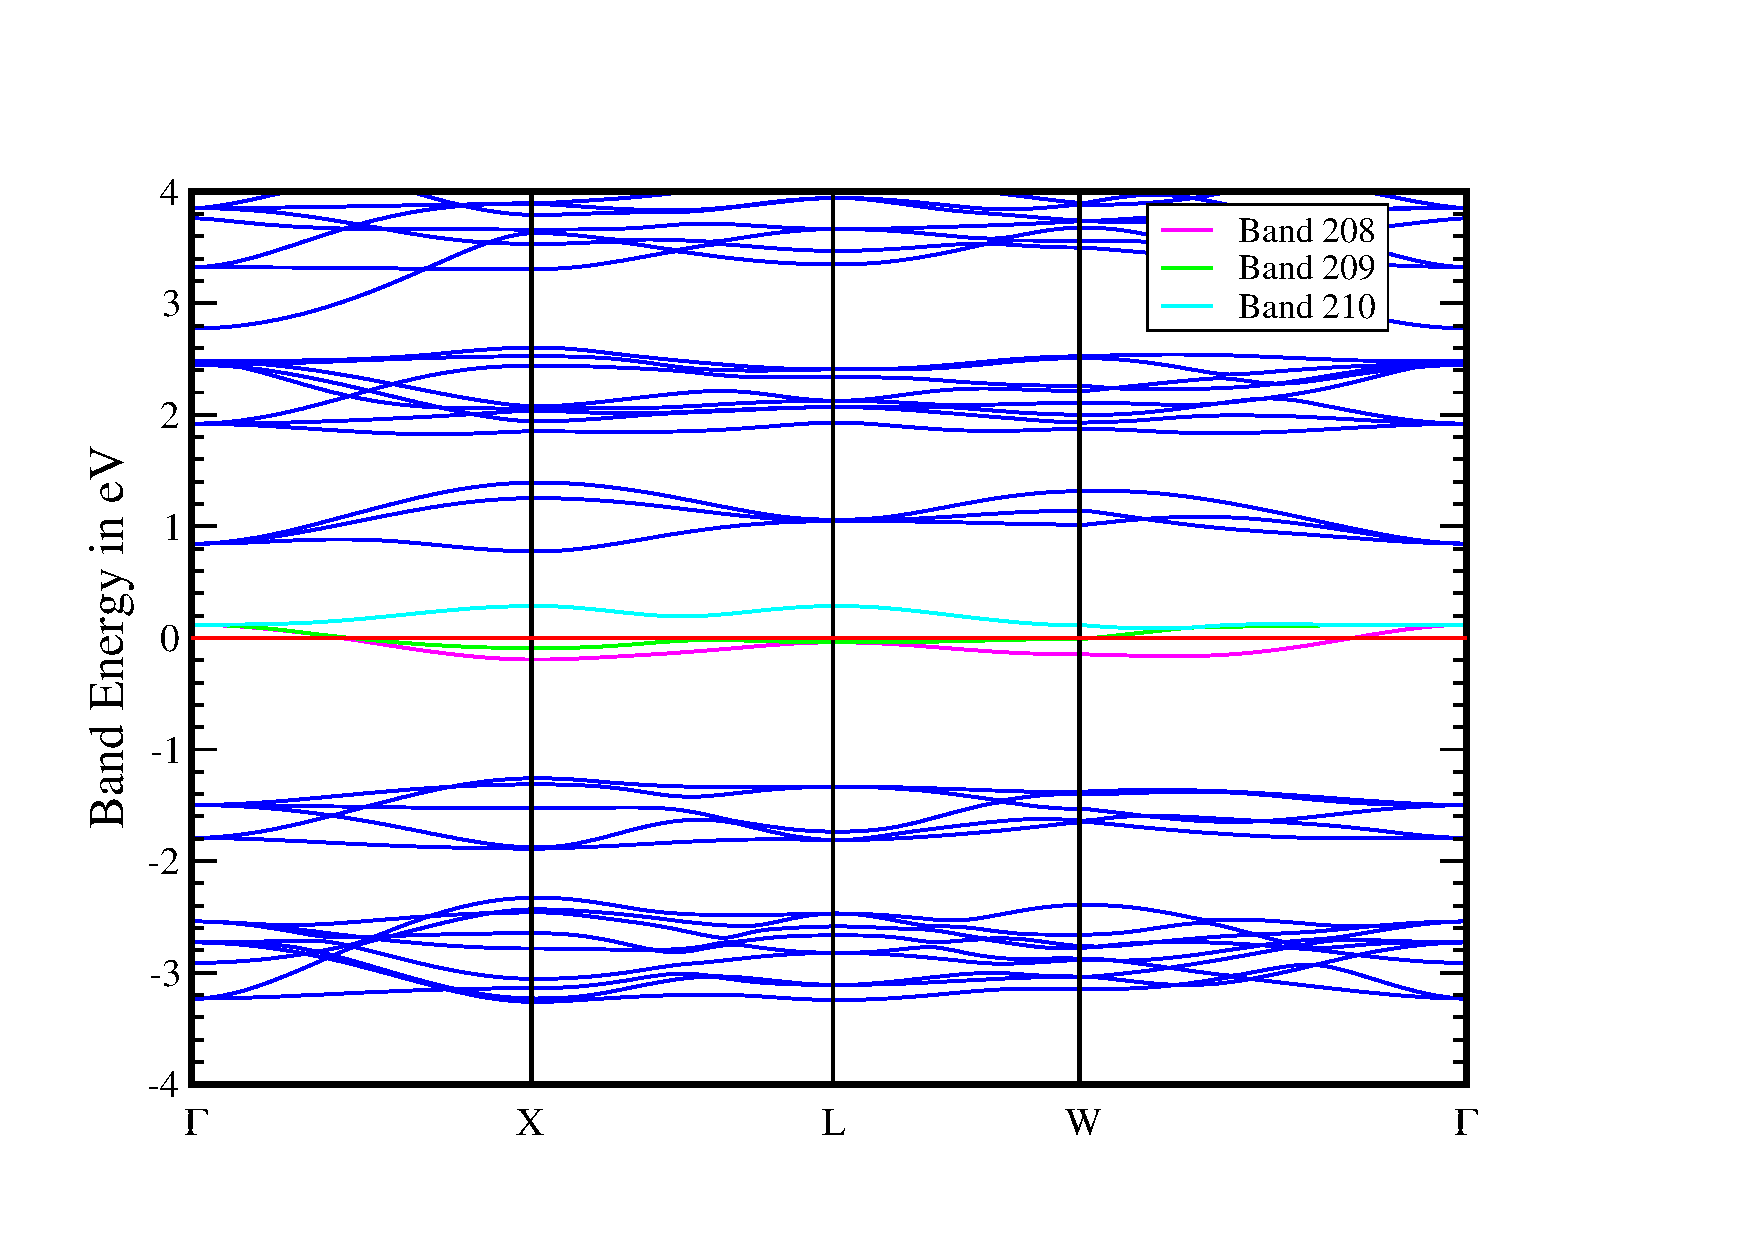
\includegraphics[width=\linewidth]{K3C60-bands.pdf}
\end{minipage}\hfill
\begin{minipage}{0.48\linewidth}
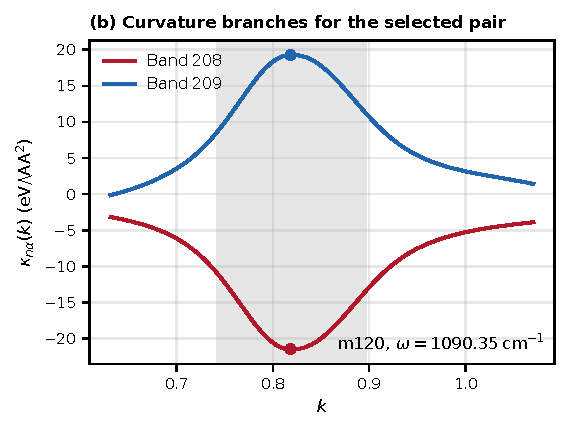
\includegraphics[width=\linewidth]{figure2_k3c60_panel_b_curvature.pdf}
\end{minipage}

\vspace{0.5em}

\begin{minipage}{0.48\linewidth}
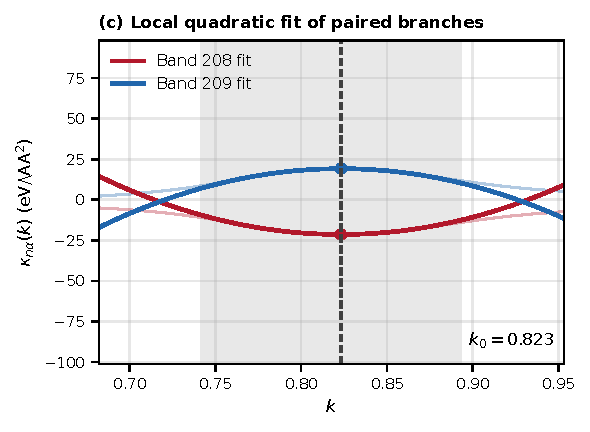
\includegraphics[width=\linewidth]{figure2_k3c60_panel_c_fit.pdf}
\end{minipage}\hfill
\begin{minipage}{0.48\linewidth}
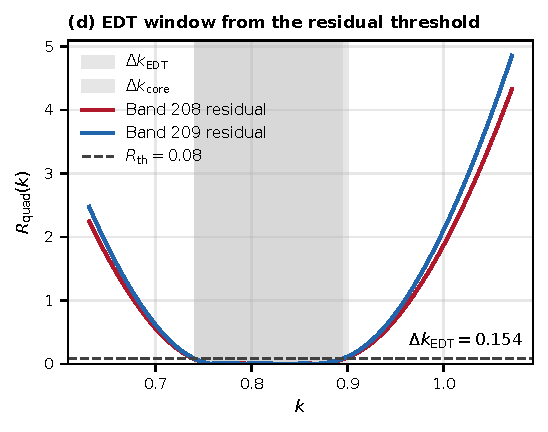
\includegraphics[width=\linewidth]{figure2_k3c60_panel_d_window.pdf}
\end{minipage}

\vspace{0.5em}

\begin{minipage}{0.48\linewidth}
\centering
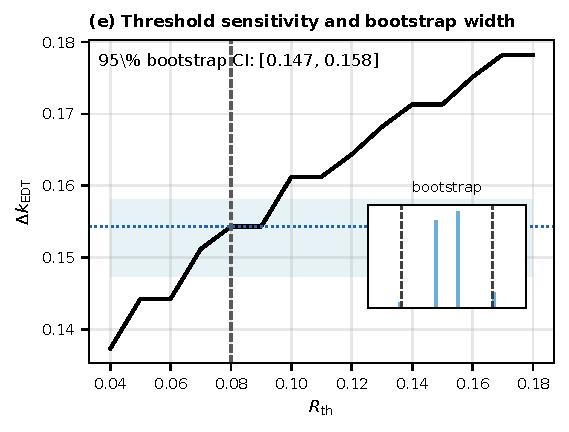
\includegraphics[width=\linewidth]{figure2_k3c60_panel_e_bootstrap.pdf}
\end{minipage}
\caption{\textbf{Curvature-defined EDT window in K$_3$C$_{60}$.}
(a) Near-Fermi band-structure context for cubic K$_3$C$_{60}$ from the archived companion band plot of the same calculation. (b) Mode-resolved curvature $\kappa_{n\alpha}(k)$ for the selected paired branches, Bands 208 and 209, for mode \texttt{m120} at $1090.35~\mathrm{cm}^{-1}$. (c) Local quadratic fits for the paired branches, yielding a shared center near $k_0=0.823$. (d) Branch-resolved normalized residuals and the nominal EDT window extracted at $R_{\rm th}=0.08$, giving $\Delta k_{\rm EDT}=0.154$. (e) Threshold sensitivity of the extracted width together with a local-fit bootstrap inset. Panels (b)--(e) are generated from \texttt{data/k3c60/tmp.agr} by \texttt{scripts/make\_fig2\_k3c60\_edt.py}.}
\label{fig:k3c60_edt_window}
\end{figure*}
